%% ----------------------------------------------------------------
%% AppendixC.tex
%% ---------------------------------------------------------------- 


%\chapter{Something} \label{Chapter:Something}
\section{Additional Notes} \label{Section:Notes}


	\begin{figure}[ht!]
		\centering
		%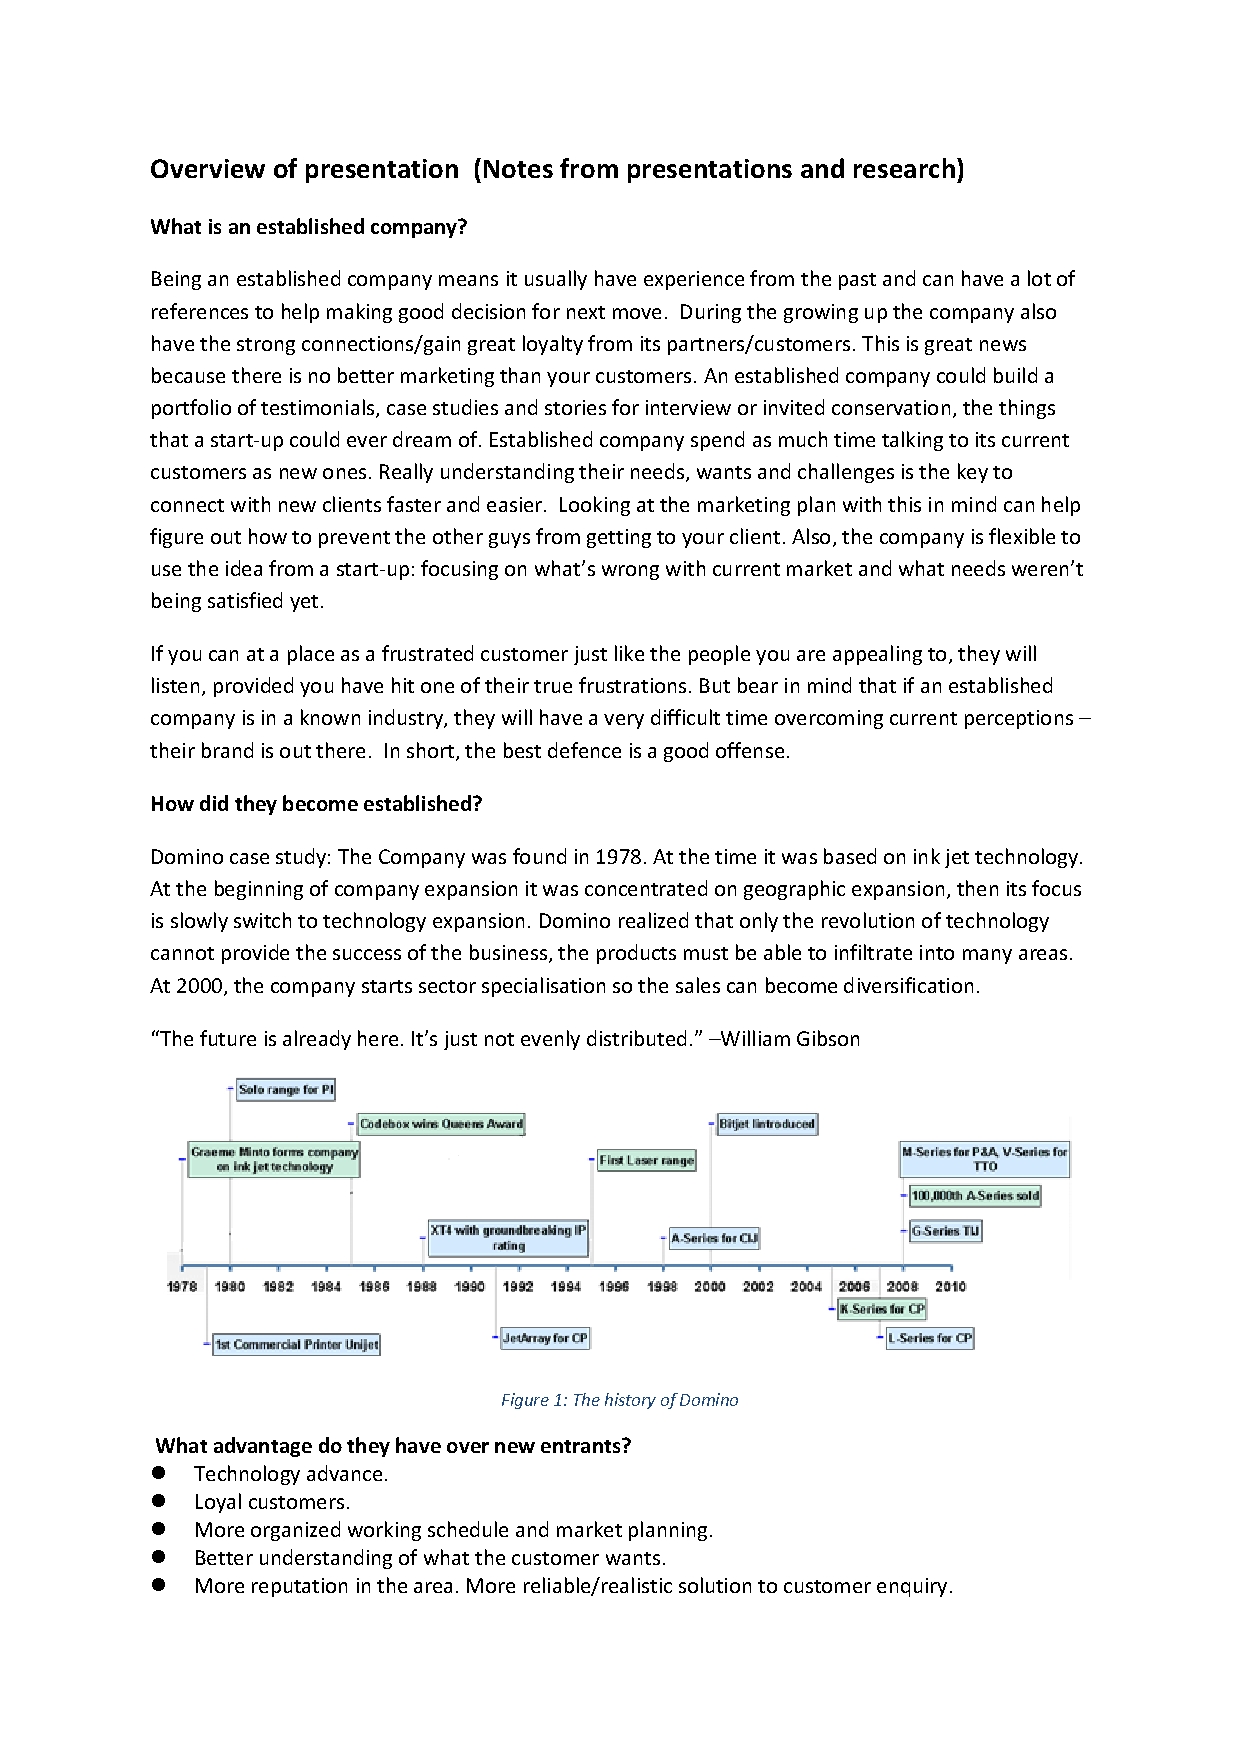
\includegraphics[width = 0.9\textwidth]{Figures/Overview_of_presentations}
		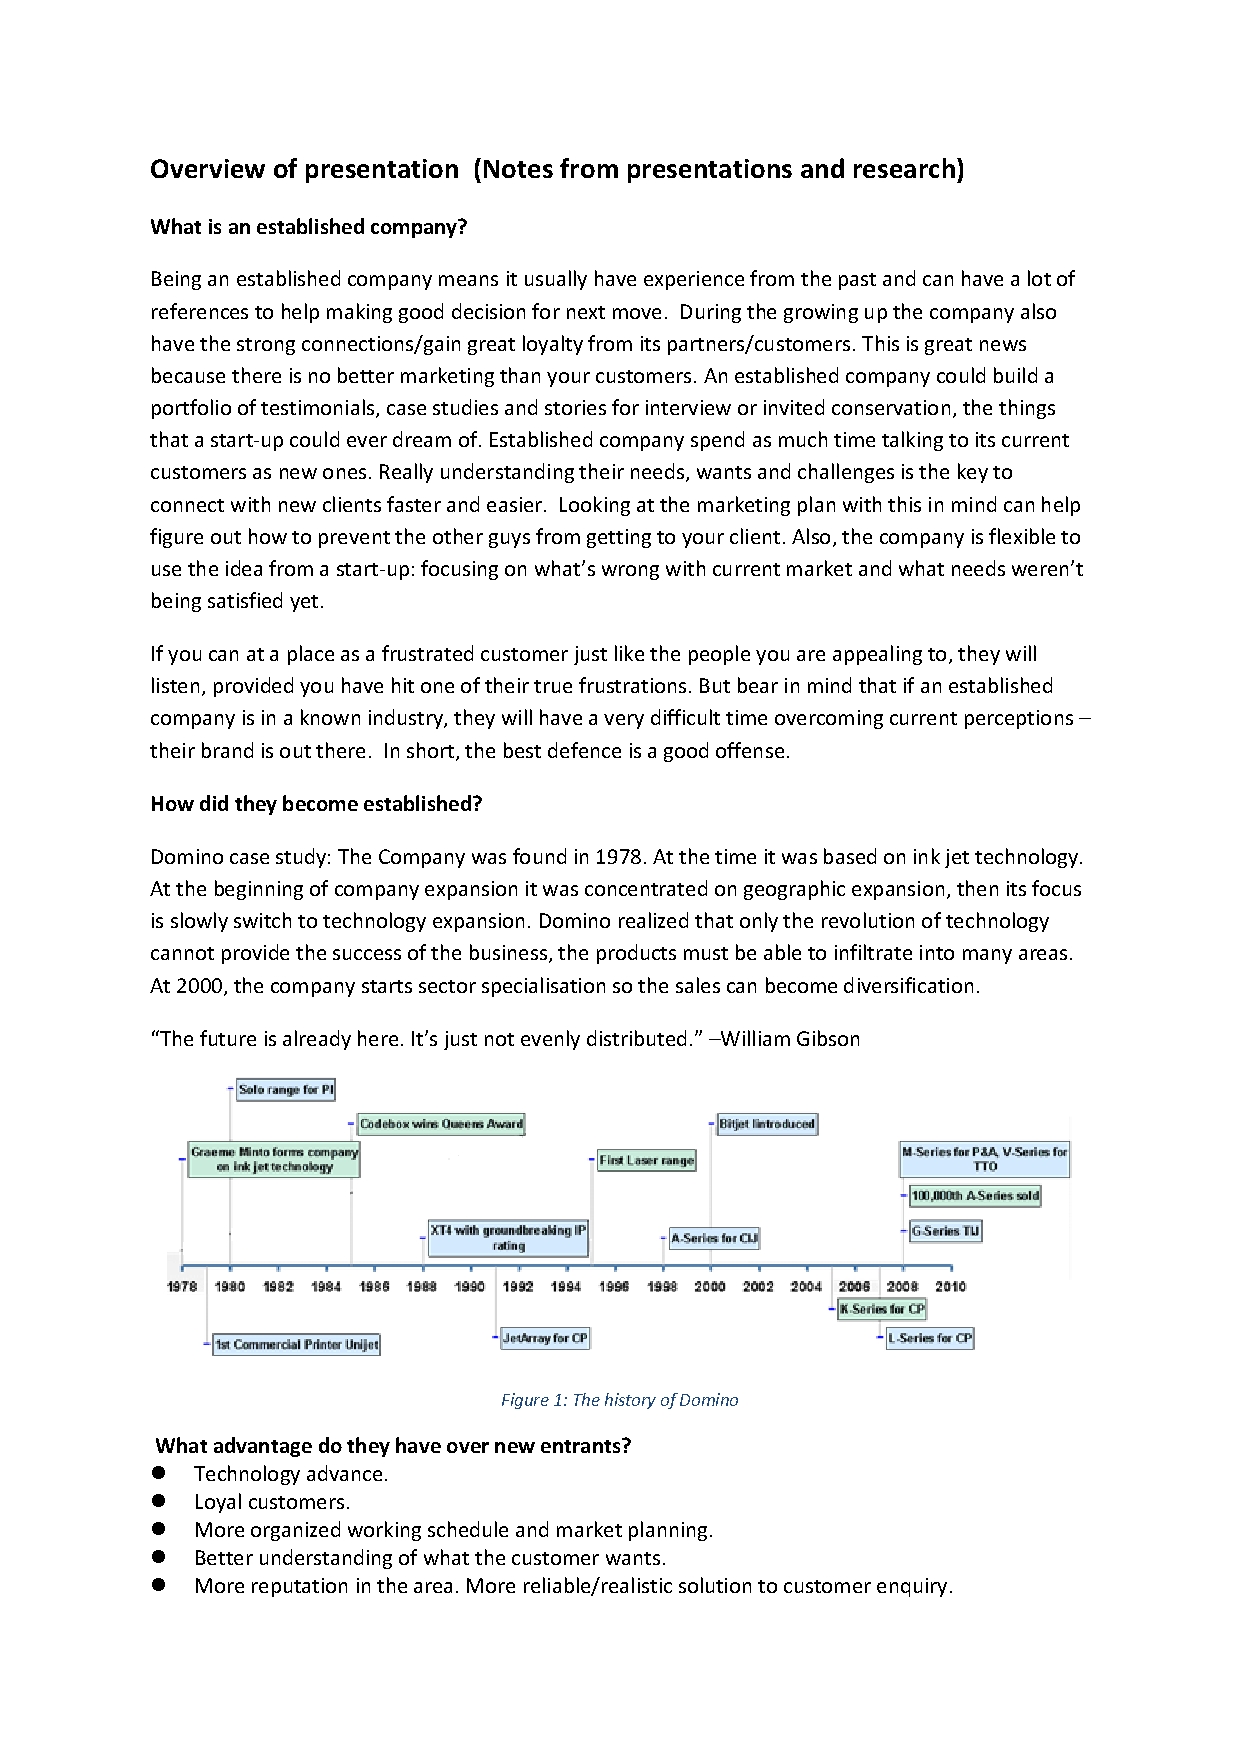
\includegraphics[width = 0.9\textwidth, page=1]{Figures/Overview_of_presentations}		
		%\caption[Additional Notes]{Notes taken for given presentations and independent research}
		\label {fig:additional:notes1}
	\end{figure}
	
		\begin{figure}[ht!]
		\centering
		%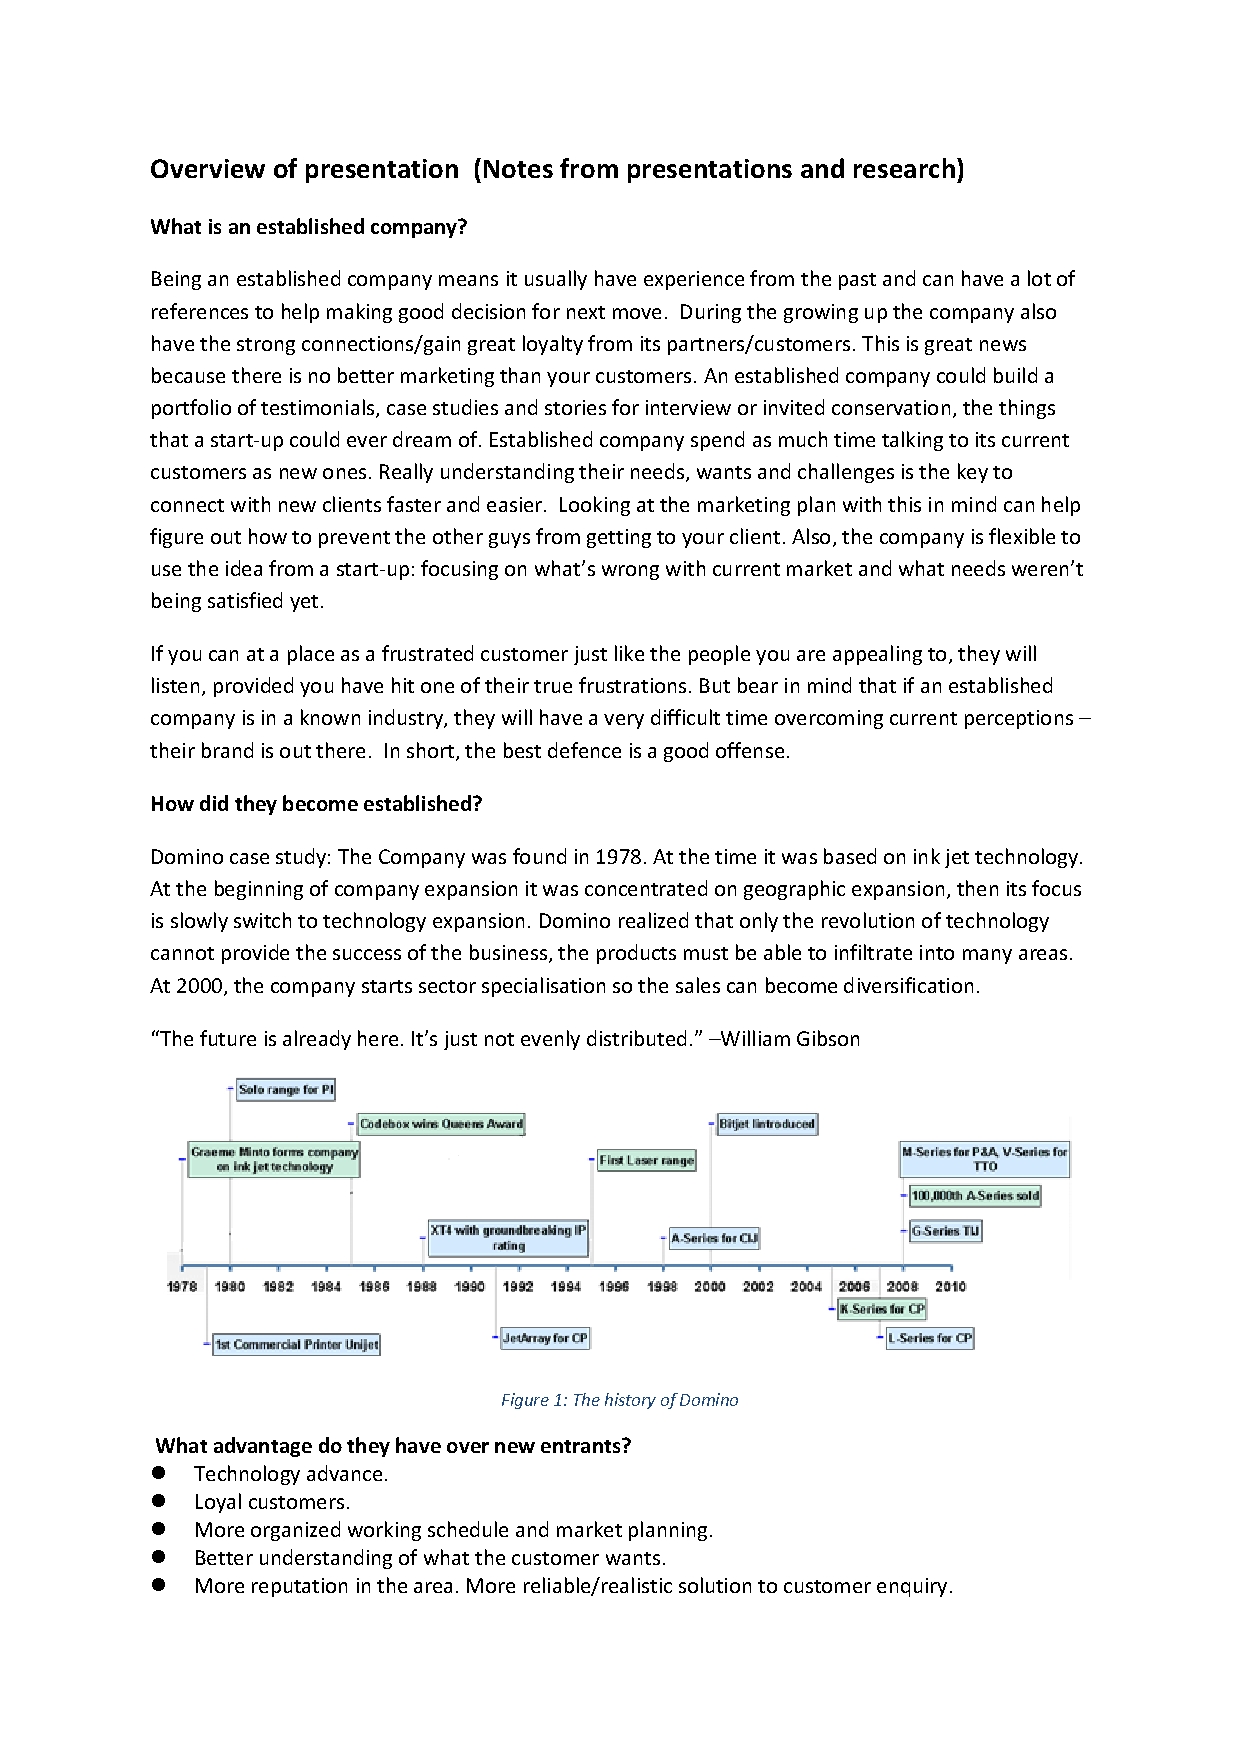
\includegraphics[width = 0.9\textwidth]{Figures/Overview_of_presentations}
		\includegraphics[width = \textwidth, page=2]{Figures/Overview_of_presentations}		
		%\caption[Additional Notes]{Notes taken for given presentations and independent research}
		\label {fig:additional:notes2}
	\end{figure}
	
		\begin{figure}[ht!]
		\centering
		%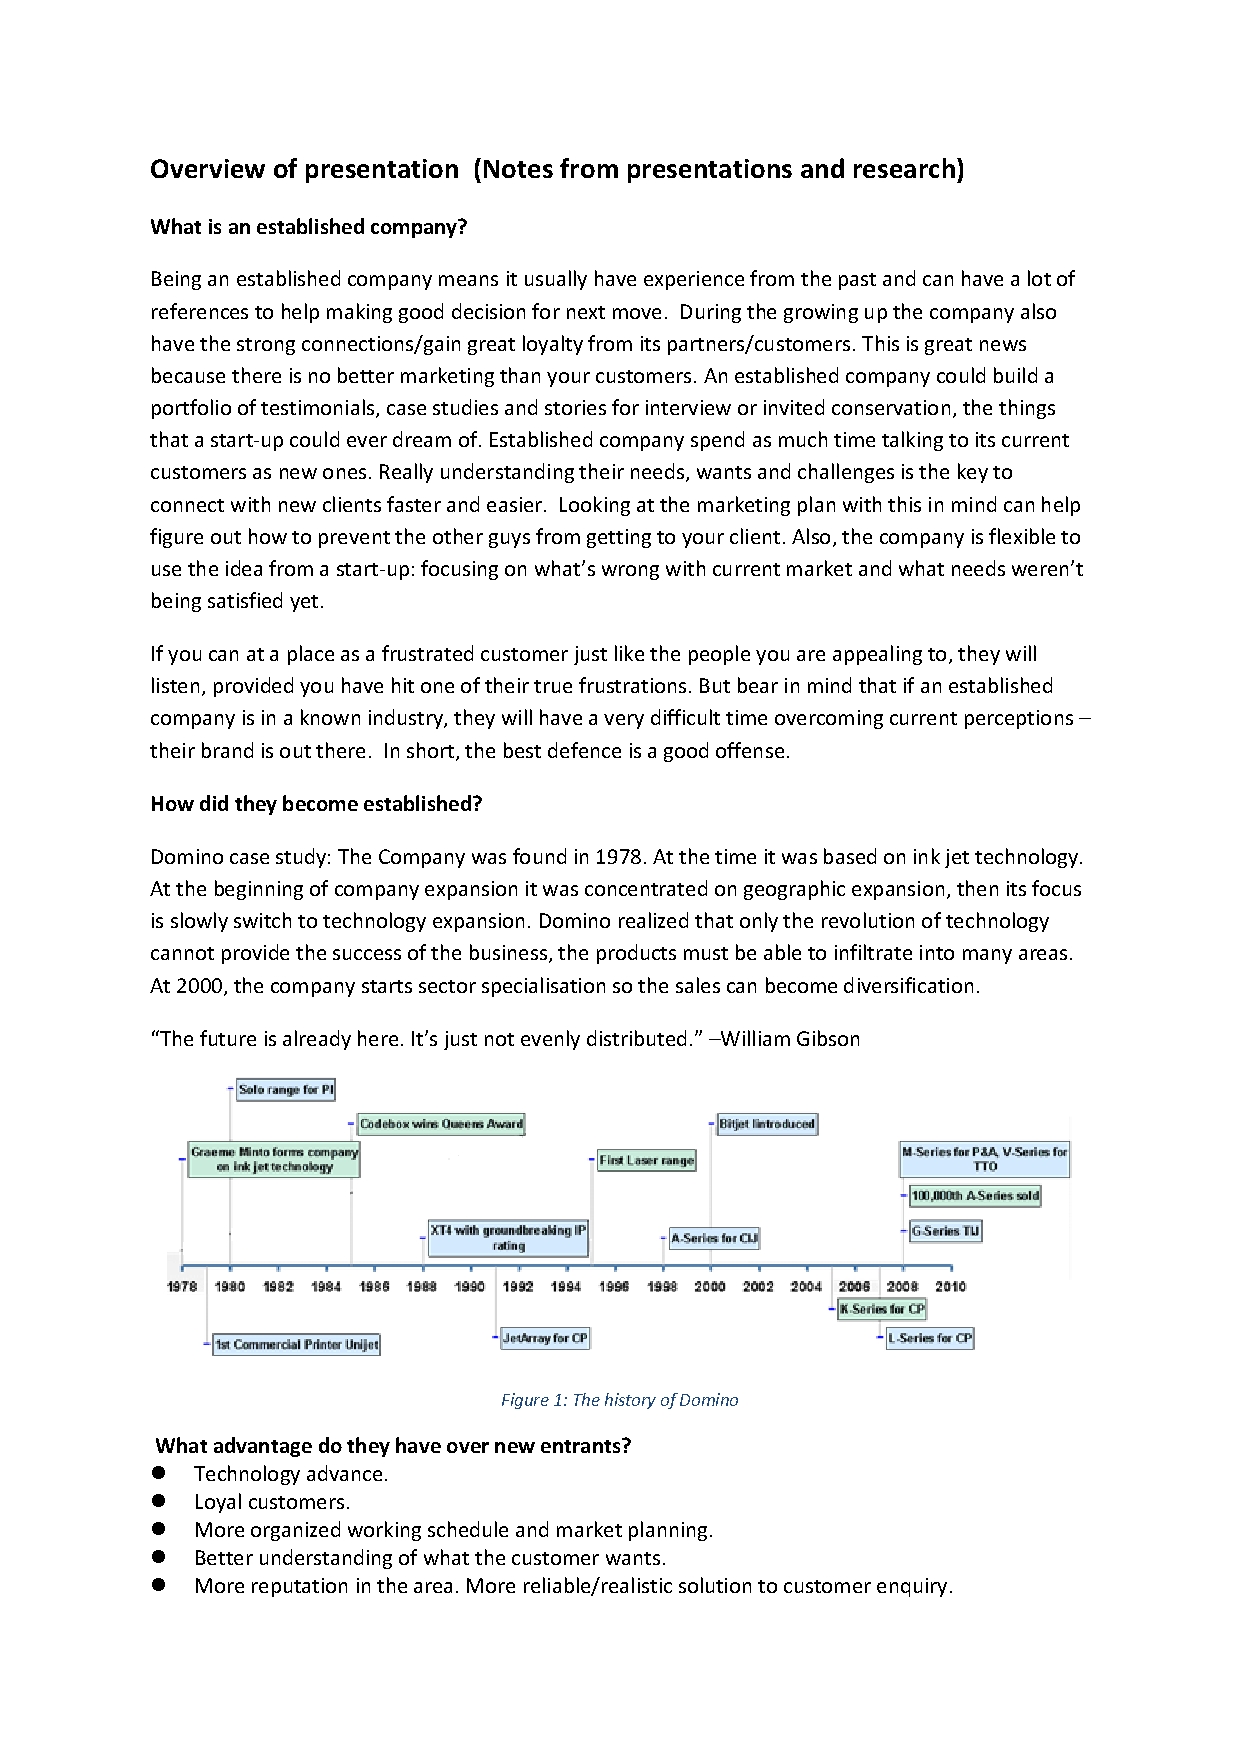
\includegraphics[width = 0.9\textwidth]{Figures/Overview_of_presentations}
		\includegraphics[width = \textwidth, page=3]{Figures/Overview_of_presentations}		
		%\caption[Additional Notes]{Notes taken for given presentations and independent research}
		\label {fig:additional:notes3}
	\end{figure}
	
		\begin{figure}[ht!]
		\centering
		%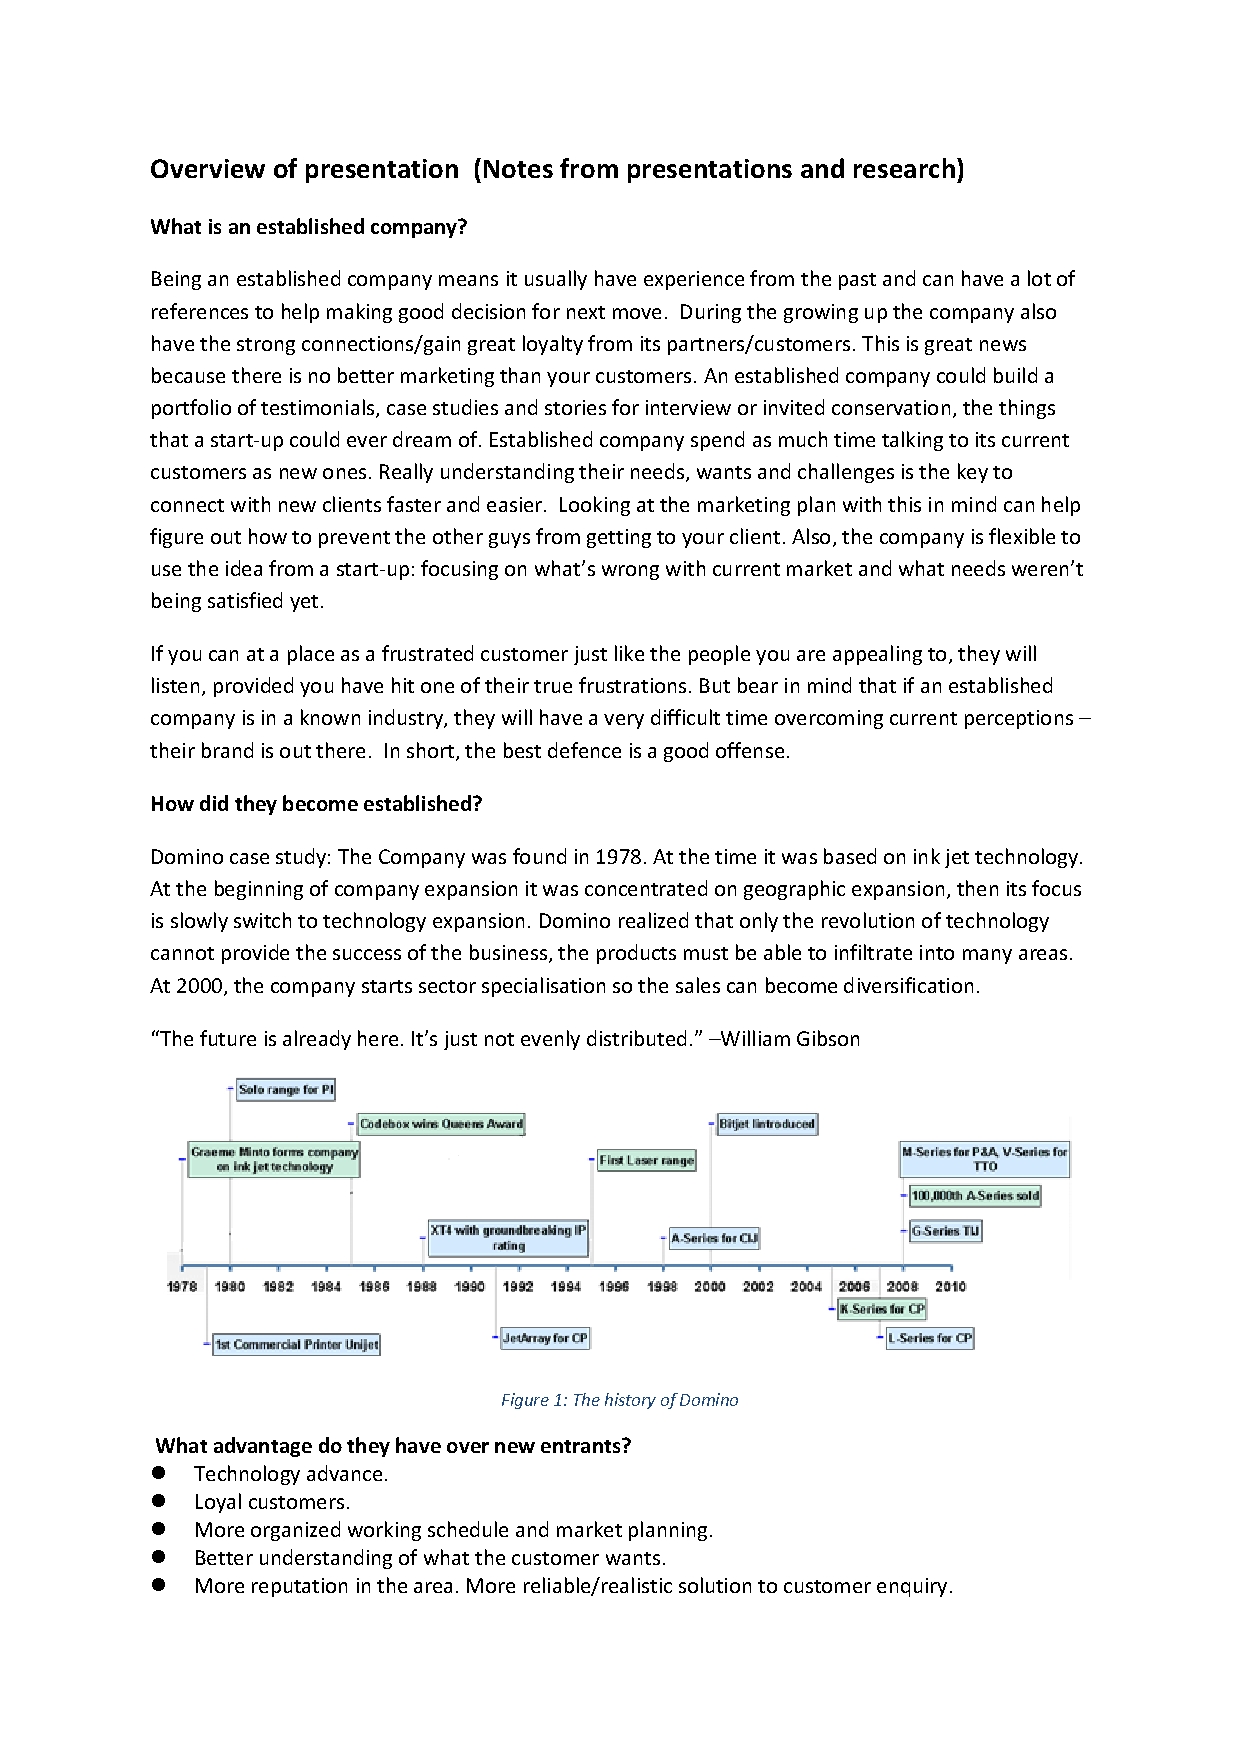
\includegraphics[width = 0.9\textwidth]{Figures/Overview_of_presentations}
		\includegraphics[width = \textwidth, page=4]{Figures/Overview_of_presentations}		
		%\caption[Additional Notes]{Notes taken for given presentations and independent research}
		\label {fig:additional:notes4}
	\end{figure}
	
		\begin{figure}[ht!]
		\centering
		%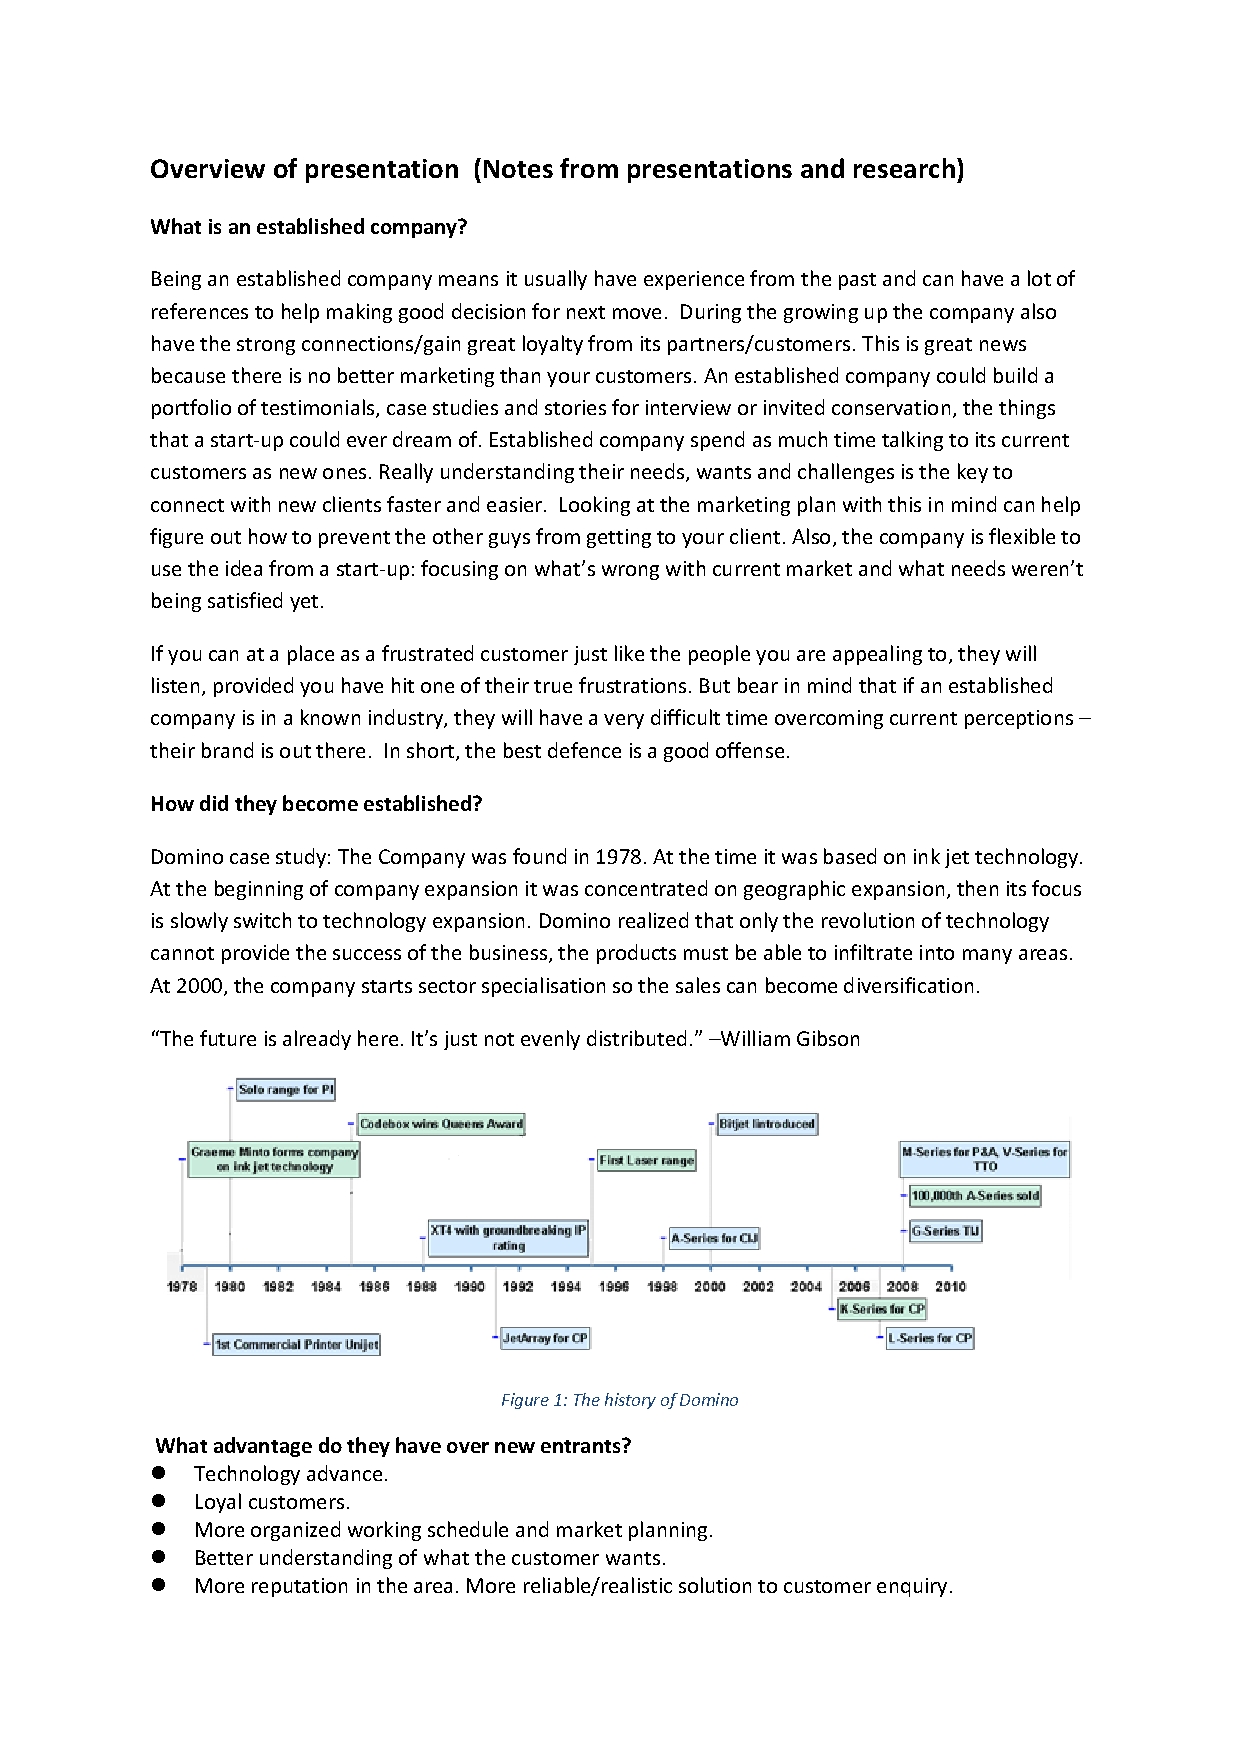
\includegraphics[width = 0.9\textwidth]{Figures/Overview_of_presentations}
		\includegraphics[width = \textwidth, page=5]{Figures/Overview_of_presentations}		
		\caption[Additional Notes]{Notes taken for given presentations and independent research}
		\label {fig:additional:notes5}
	\end{figure}